In this chapter the planning and work-flow regarding Sprint 2 will be described. 
Everything from setting the goals to implementation, and testing. At the end there will evaluate whole sprint, and answers to following questions: What went well? What could be improved? What should we start doing? 

\section{Sprint planning}
The customer was very satisfied with the demonstration video for sprint 1, and suggested recording future prototypes as well. 
After the successful sprint 1 review, the planning of next sprint was started. 
Since the customer was very happy with the sprint 1 delivery, he gave the team an opportunity to decide for themselves what they want to work on in sprint 2, and then ask for his approval.
It has been decided by the team to focus on multiple client support, and since sprint 1 just focused on connecting one client to the server, then it would also be a good opportunity to refine the code which was implemented so far. 
The customer thought this was a really good idea, because working on this now could help in future. 
Catching problems in early phases is much better than discovering them too close to the deadline. 
Then it might not be possible to have enough time to fix those problems.
Therefore sprint 2 will focus on adding support for multiple clients connection and sending different signals to different clients. 
Existing code should be revised and improved so that in next sprint the main effort can be focused on image processing module.


In the supervisor meeting the day after the sprint review, the project report draft was shown to supervisor. 
He was satisfied with the new structure, but he wanted the team to finish more sections. He also insists on creating a work break down structure for the project. 
There were also some chapters that could be merged, which means we should refine the structure of the report. 
These suggestions were included into the sprint plan and according to time estimation some stories were adjusted.

\subsection{Duration}
This Sprint will be 2 weeks long. From 16.09.2013 to 29.09.2013.
The team agreed on the date of presentation and showing the running demo -- Thursday 26.09.2013.
Estimated velocity is 240h since team agreed on 30 working hours per person per week.

\subsection{User-stories}

\subsubsection*{Implementation}
All the functional requirements for sprint 2 are presented in Table \ref{tab:sprint2stories}
\LTXtable{\textwidth}{sprint2/stories.tex}

\subsubsection*{Documentation}
All the documentation stories for sprint 2 are presented in Table \ref{tab:sprint2Documentationstories}
\LTXtable{\textwidth}{sprint2/storiesDocumentation.tex}

\subsubsection*{Project management}
All the project management stories for sprint 2 are presented in Table \ref{tab:sprint2storiesProcess}
\LTXtable{\textwidth}{sprint2/storiesProcess.tex}

% hous all in total: Estimated: 57+104+50= 211 Spent: 48+102 +43 = 193
\section{Sprint Goals}
The goal for Sprint 2 is to deliver a working demo with a more refined core client-server module. 
This still includes registering services, listening for the client and sending simple signals to the client from the server application, but with a more refined code. 
Of course the client should still scan for the services, connect, receive signals, and play the commands. 
The goal is still to use the established simple communication protocol. 
All of the above is extended so it works for several clients connected to the server.

Goals about the report are to refine the report and write the sections needed to be up to speed with the report. This means that sprint 1 chapter has to be finished same as sprint 2 chapter. 

\section{System Burndown}
\begin{figure}[H]
	\centering
		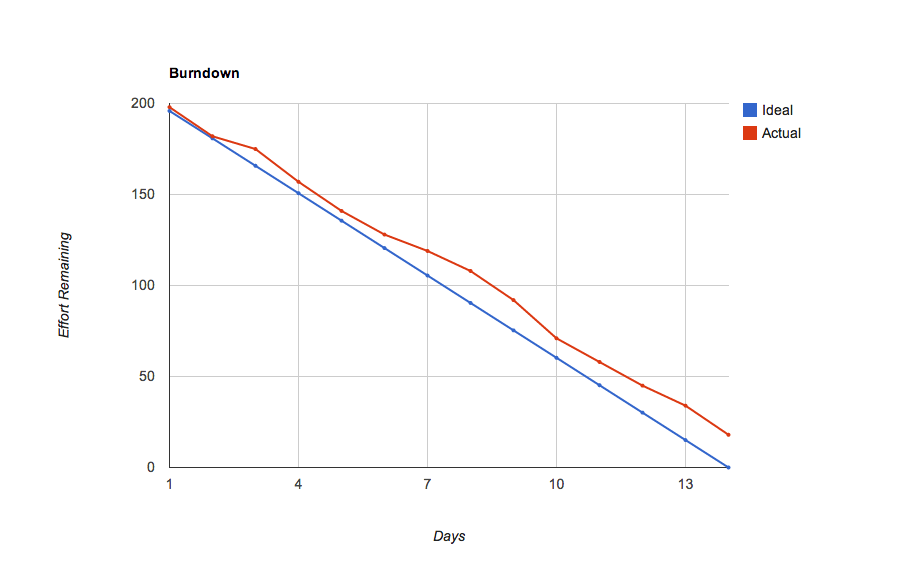
\includegraphics[width=18cm]{sprint2/BurndownSprint2.png}
	\caption{Burn down chart}
	\label{fig:Burn2 }
\end{figure}

\section{Architecture}
\section{Implementation}
\section{Testing}
\section{Occurring risks}

The risk table \ref{tab:risks} shows many different risks that can occur. 
For this sprint most of them did not occur. 
This is because the most challenging technical parts are not developed yet. 
This is scheduled for sprint 3. 

The user stories for this sprint were also very clear, and really not that different from the last sprint. 
The only difference was that instead of one client, there are now several clients connected to the server. 
As mentioned earlier the customer was very happy with the demonstration in sprint 1, and he let the team choose the stories for this sprint. 
He approved the chosen stories, and because of this no changes in requirements were not met in the last minute.
 
In this sprint the team also did a better job with the time estimation. 
All of this avoids a lot of issues, which is advantage. 
  
\section{Customer feedback}

\section{Retrospective}
This section reflects on the past sprint. In order to learn from the mistakes done and thus to improve the workflow it is necessary to answer two essential questions: "What went well" and "What could be improved".

\subsection{What went well}
The team reached the sprint 2 goals. 
The team delivered the demo with more refined code, and as planned this code supported multiple clients. 
The clients were able to play the commands the server sent.
Another milestone was reached -- Obedient crowd -- Prototype 2.

The work done in the report is very good -- the report is better structured now.
Some extra hours were spent on going through the whole report. 
This was to see if we need to add more in the specific sections, or if we should remove something.  

Even though some members had other responsibilities, and had to absent in some of the working hours, the team still got everything from implementation part done in time for the sprint review. Everyone worked really well independently, as well as in team. 

%The sprint planning in this sprint went really well. 
%We had a perfect amount of work, and the hours estimated for each task, was very realistic, so that was good. 


\subsection{What could be improved}
%The time tracking of each task could have been done better. 
%Even though the team members track their own time, the TargetProcess3 program dos not have a feature for manually edit the time tracking. 
%This means if we forget to do it right away, then the burn down chart wont be as reliable. 
%Since this shows our time tracking we should try to be better at that.

When there is work that needs to be done in the report, the person who writes this section should read terminology, or what other team members have written earlier. 
This will help to get a better flow for the reader.
This will also save a couple of hours when refining is needed afterwards. 
